\section{Assessment of the different approaches}

Based on our reference measurements from the section \ref{sec:reference}, we can assess the performances of our two different approaches.
To determine which approach perform the best, the difference between the measured context switching time and the real one is used.
Moreover, comparing the distributions of the measurements can refine the analysis.

\subsection{Extension approach performance}

For our extension approach, we can say that it performs poorly.
For example, on Contiki with the RE-Mote board, the expected context switching time is 18.505 $\mu$s but our framework measured a context switching time of 31.6162 $\mu$s.
This represents a difference of $70\%$.

The real-time clock used to measure the context switching time is not precise enough.
This lack of precision explains the framework results.
During our experiments, we have noticed that on the Z1 board, the real-time clock has a speed of 32768 ticks per second.
In other words, a tick occurs every 30.5 $\mu$s.
This is why the minimal value measured with Contiki on the Z1 board is 30.5175 $\mu$s.
The same logic can be applied with RIOT or the RE-Mote board.

With a slow clock, it is not possible to have precise measures for the context switching time.
Unfortunately, we did not find any solution to overcome this problem.
Therefore, it is not possible to compute the context switching time internally.

\subsection{Devices approach performance}

With the devices approach, we have better results than with our first framework.
First, the measurements done with the framework differ only by 2.8\% with both Contiki and RIOT.

Wuth Contiki, we have a maximum difference of 0.5 $\mu$s with the reference value.
When comparing the distributions of the framework measurements with the distributions of the reference measurements, we can see that they match.
The figure \ref{fig:comparison-devices-framework-contiki-remote} shows the distributions comparison with measurements made on the RE-Mote board.

\begin{figure}[!ht]
  \centering
  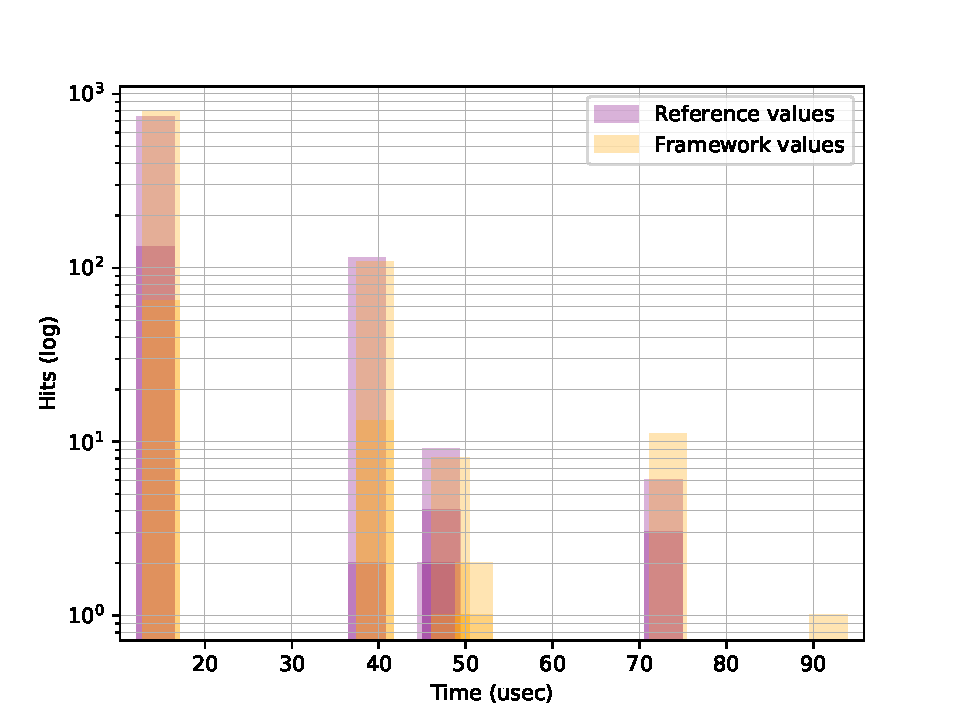
\includegraphics[scale=.7]{assets/comparison-devices-framework-contiki-remote.pdf}
  \caption{distributions comparison with Contiki on the RE-Mote board\label{fig:comparison-devices-framework-contiki-remote}}
\end{figure}

The figure \ref{fig:comparison-devices-framework-contiki-z1} shows the distributions comparison with measurements made on the Z1 board.

\begin{figure}[!ht]
  \centering
  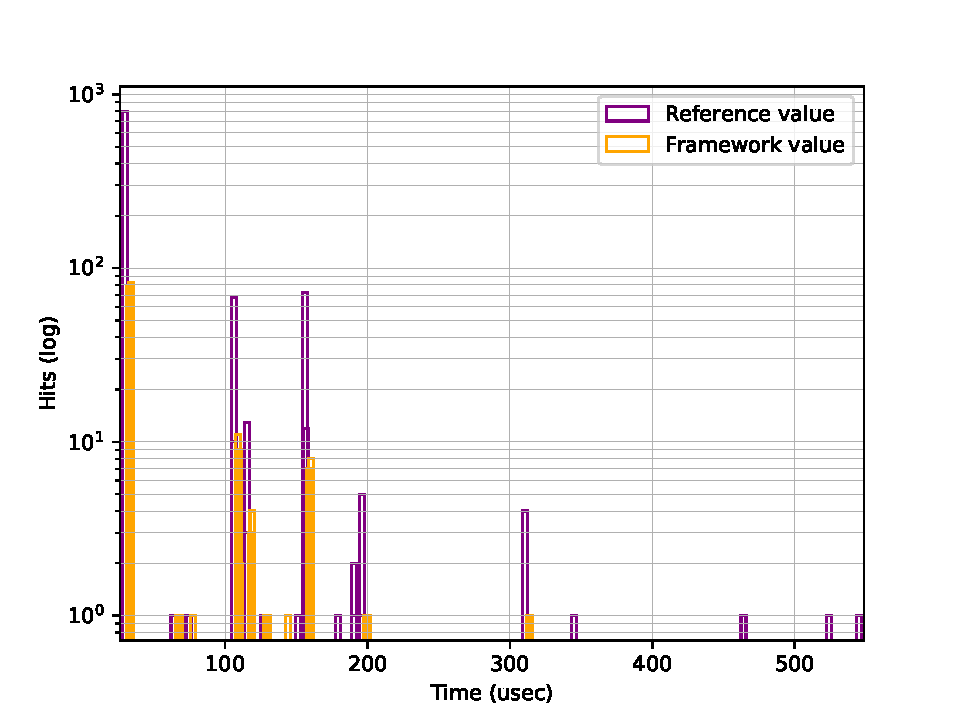
\includegraphics[scale=.7]{assets/comparison-devices-framework-contiki-z1.pdf}
  \caption{distributions comparison with Contiki on the Z1 board\label{fig:comparison-devices-framework-contiki-z1}}
\end{figure}

With RIOT, we have a maximum difference of 3 $\mu$s.
With the RE-Mote board, the difference between the real context switching time and the measurements made by the framework is 0.35 $\mu$s.
In the other hand, with the Z1 board, this difference is 2.99 $\mu$s.
We were not able to determine from where this difference comes from.
However, by comparing the measurements distributions, we see a strong correlation between the reference measurements and the framework measurements.

The figure \ref{fig:devices-comparison-riot-remote} shows the distributions comparison with measurements made on the RE-Mote board and the figure \ref{fig:devices-comparison-riot-z1} shows the same comparison but on the Z1 board.

\begin{figure}[!ht]
  \centering
  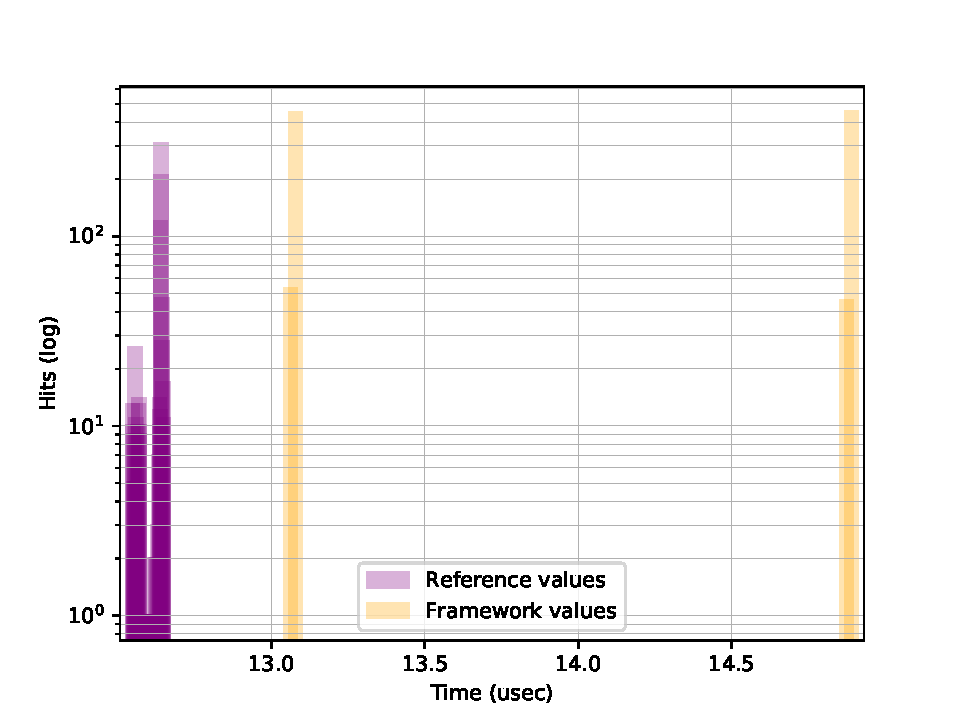
\includegraphics[scale=.7]{assets/comparison-devices-framework-riot-remote.pdf}
  \caption{distributions comparison with RIOT on the RE-Mote board\label{fig:devices-comparison-riot-remote}}
\end{figure}

\begin{figure}[!ht]
  \centering
  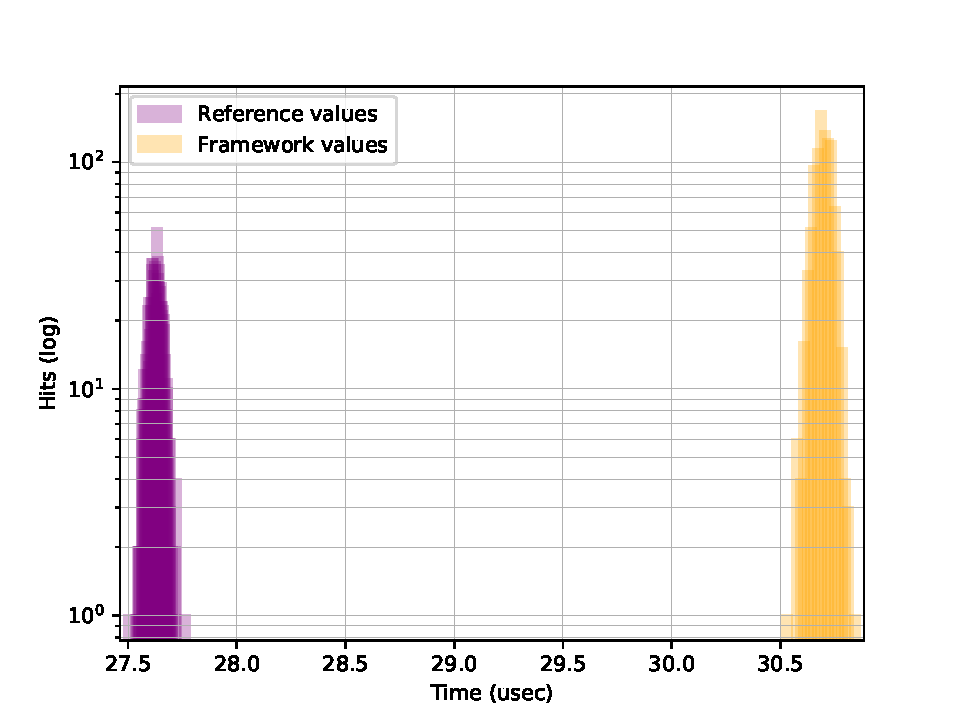
\includegraphics[scale=.7]{assets/comparison-devices-framework-riot-z1.pdf}
  \caption{distributions comparison with RIOT on the Z1 board\label{fig:devices-comparison-riot-z1}}
\end{figure}